% 
% Lecture Template for ME3050 -  Dynamics Modeling and Controls - Tennessee Technological University
%
% Spring 2020 - Summer 2020
% Tristan Hill, May 07, 2020
% Dyanmics Review - Topic 4 - Particles and Bodies
%

\documentclass{beamer}                         % for presentation (has nav buttons at bottom)
%\documentclass[handout]{beamer}  % for handout 
\usepackage{beamerthemesplit}
\usepackage{amsmath}
\usepackage{listings}
\usepackage{multicol}

\beamertemplateballitem

\definecolor{TTUpurple}{rgb}{0.3098, 0.1607, 0.5176} % TTU Purple (primary)
\definecolor{TTUgold}{rgb}{1.0000, 0.8666, 0.0000} % TTU Gold (primary)

\setbeamercolor{palette primary}{bg=TTUpurple,fg=TTUgold}
\setbeamercolor{palette secondary}{bg=black,fg=TTUgold}
\setbeamercolor{palette tertiary}{bg=black,fg=TTUpurple}
\setbeamercolor{palette quaternary}{bg=TTUgold,fg=black}
\setbeamercolor{structure}{fg=TTUpurple} % itemize, enumerate, etc
\setbeamercolor{section in toc}{fg=TTUpurple} % TOC sections

%\usefonttheme{professionalfonts}

\newcommand{\LNUM}{2\hspace{2mm}} % Lecture Number 

\newcommand{\Lagr}{\mathcal{L}} % lagrangian

\newcommand{\vspccc}{\vspace{6mm}\\} % large vertical space
\newcommand{\vspcc}{\vspace{4mm}\\}   % medium vertical space
\newcommand{\vspc}{\vspace{2mm}\\}     % small vertical space

\newcommand{\hspcccc}{\hspace{10mm}} % large horizontal space
\newcommand{\hspccc}{\hspace{6mm}} % large horizontal space
\newcommand{\hspcc}{\hspace{4mm}}   % medium horizontal space
\newcommand{\hspc}{\hspace{2mm}}     % small horizontal space


\author{ME3050 - Dynamics Modeling and Controls} % original formatting from Mike Renfro, September 21, 2004

\newcommand{\TNUM}{4\hspace{2mm}} % topic Number 
\newcommand{\firsttitle}{Dynamics Review - Topic \TNUM} % first line of title (used by beamer)
\newcommand{\secondtitle}{Particles and Bodies}% second line of the title of this presentation (used by TWH)

\title{\firsttitle}

\date{May 29, 2020}

\begin{document}

\lstset{language=MATLAB,basicstyle=\ttfamily\small,showstringspaces=false}

% Section 0: Outline
\frame{\titlepage \center\textbf{\secondtitle}\vspace{5mm}\\}

\frame{

\large \textbf{Lecture \LNUM - \secondtitle} \vspace{3mm}\\

%Topics : \vspace{3mm}\\ % ' topics' are beamer 'sections' - TWH

\begin{itemize}
	\item What is a Rigid Body?\vspace{3mm}\\ % Section 1
	\item Mathematical Definition of Rigid Body Motion\vspace{3mm}\\% Section 2
	\item Is rigid body motion realistic?\vspace{3mm}\\ %Section 3
	\item Examples\vspace{3mm}\\ % Section 4
	%\item Example\vspace{3mm}\\ % Section 5 - 5 is almost too many...
\end{itemize}
}

% Section 1: What is a Rigid Body?
\section{What is a Rigid Body?}

\frame{

  \frametitle{What is a Rigid Body?}


\begin{itemize}
\item Blah\vspace{3mm}\\
\item Blah \vspace{3mm}\\
\item Blah blah \vspace{3mm}\\
\end{itemize}

}

% Section 2: What is Dynamics?
\section{What is Dynamics?}
\frame{

\frametitle{What is Dynamics?}
\Large{"Dynamics is the study of how moving objects behave. Dynamics is the part of mechanics that studies movement and its causes. The study of the causes of motion and changes in motion is known as dynamics. Dynamics is the study of how moving objects behave."} \vspace{5mm} \\

\Large{"The dynamical system concept is a mathematical formalization for any fixed "rule" which describes the time dependence of a point's position in its ambient space. "} \vspace{5mm} \\

}

% Section 3: Dynamics in Mechanical Engineering
\section{Dynamics in Mechanical Engineering}
\frame{

\frametitle{Dynamics in Mechanical Engineering}

\Large{Why are we studying Dynamics?} \vspace{5mm} \\

}

% Section 4: Examples
\section{Examples}
\frame{

\frametitle{Examples}

\Large{Cool Stuff...} \vspace{5mm} \\

}
%	\item \textbf{ \LARGE \B Dynamic\K} \\
%			
%			\Large{"Dynamics is the study of how moving objects behave. Dynamics is the part of mechanics that studies movement and its causes. The study of the causes of motion and changes in motion is known as dynamics. Dynamics is the study of how moving objects behave."} \vspace{5mm} \\
%
%			\Large{"The dynamical system concept is a mathematical formalization for any fixed "rule" which describes the time dependence of a point's position in its ambient space. "} \vspace{5mm} \\
%
%	\item \textbf{ \Large Translational Motion } 
%\begin{itemize}
%\item Position
%\item Velocity 
%\item Acceleration \vspace{2mm}\\
%\end{itemize} 
%
%	\item \textbf{ \Large Rotational Motion }
%\begin{itemize}
%\item Position
%\item Velocity 
%\item Acceleration \vspace{2mm}\\
%\end{itemize} 		
%	
%	\item \textbf{ \Large Particle Motion } 
%\begin{itemize}
%\item What do mean by this? \vspace{2mm}\\
%\end{itemize}
%\item \textbf{ \Large Rigid-Body Motion } 
%\begin{itemize}
%\item What do mean by this specifically? Mathematically?
%\end{itemize}
%
%\newpage
%\item \textbf{ \Large Degrees of Freedom (DOF) } 
%	\begin{itemize}
%\item What does this mean? \vspace{25mm}\\
%\item Examples:
%\end{itemize}
%
%\newpage
%	\item \textbf{ \Large The \B dynamics \K are represented as ordinary \vspace{3mm}\\
%differential equations called the \\\\ \underline{\hspace{60mm}} of \underline{\hspace{60mm}}.} \vspace{2mm}\\
%
%	\item \textbf{ \Large Deriving the 	\underline{\hspace{60mm}} of \underline{\hspace{60mm}} \vspace{1mm}\\is typically done in one of two ways.} \\
%	\begin{enumerate}
%		\item Newtonian Approach - Vector Based Method \vspace{3mm}\\
%		\begin{itemize}
%\item Translational\\
%\item Rotational  \vspace{10mm}\\
%\end{itemize} 
%\item Conservation of Energy Approach - Energy Based Method \vspace{3mm}\\
%		\begin{itemize}
%\item Kinetic Energy\\
%\item Potential Energy\\  
%\end{itemize} 
%	\end{enumerate}
%
%\newpage
%
%\item \textbf{ \Large  Example:} DJI Phantom with 3-axis Camera Gimbal \\
%
%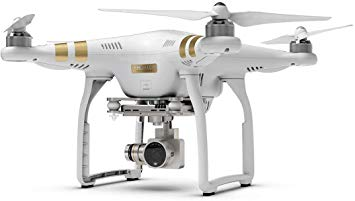
\includegraphics[scale=1]{dji_phantom.jpg}
%
%
%\newpage
%
%\item \textbf{ \Large  Simpler Example:} Quarter Car Suspension Model\\
%
%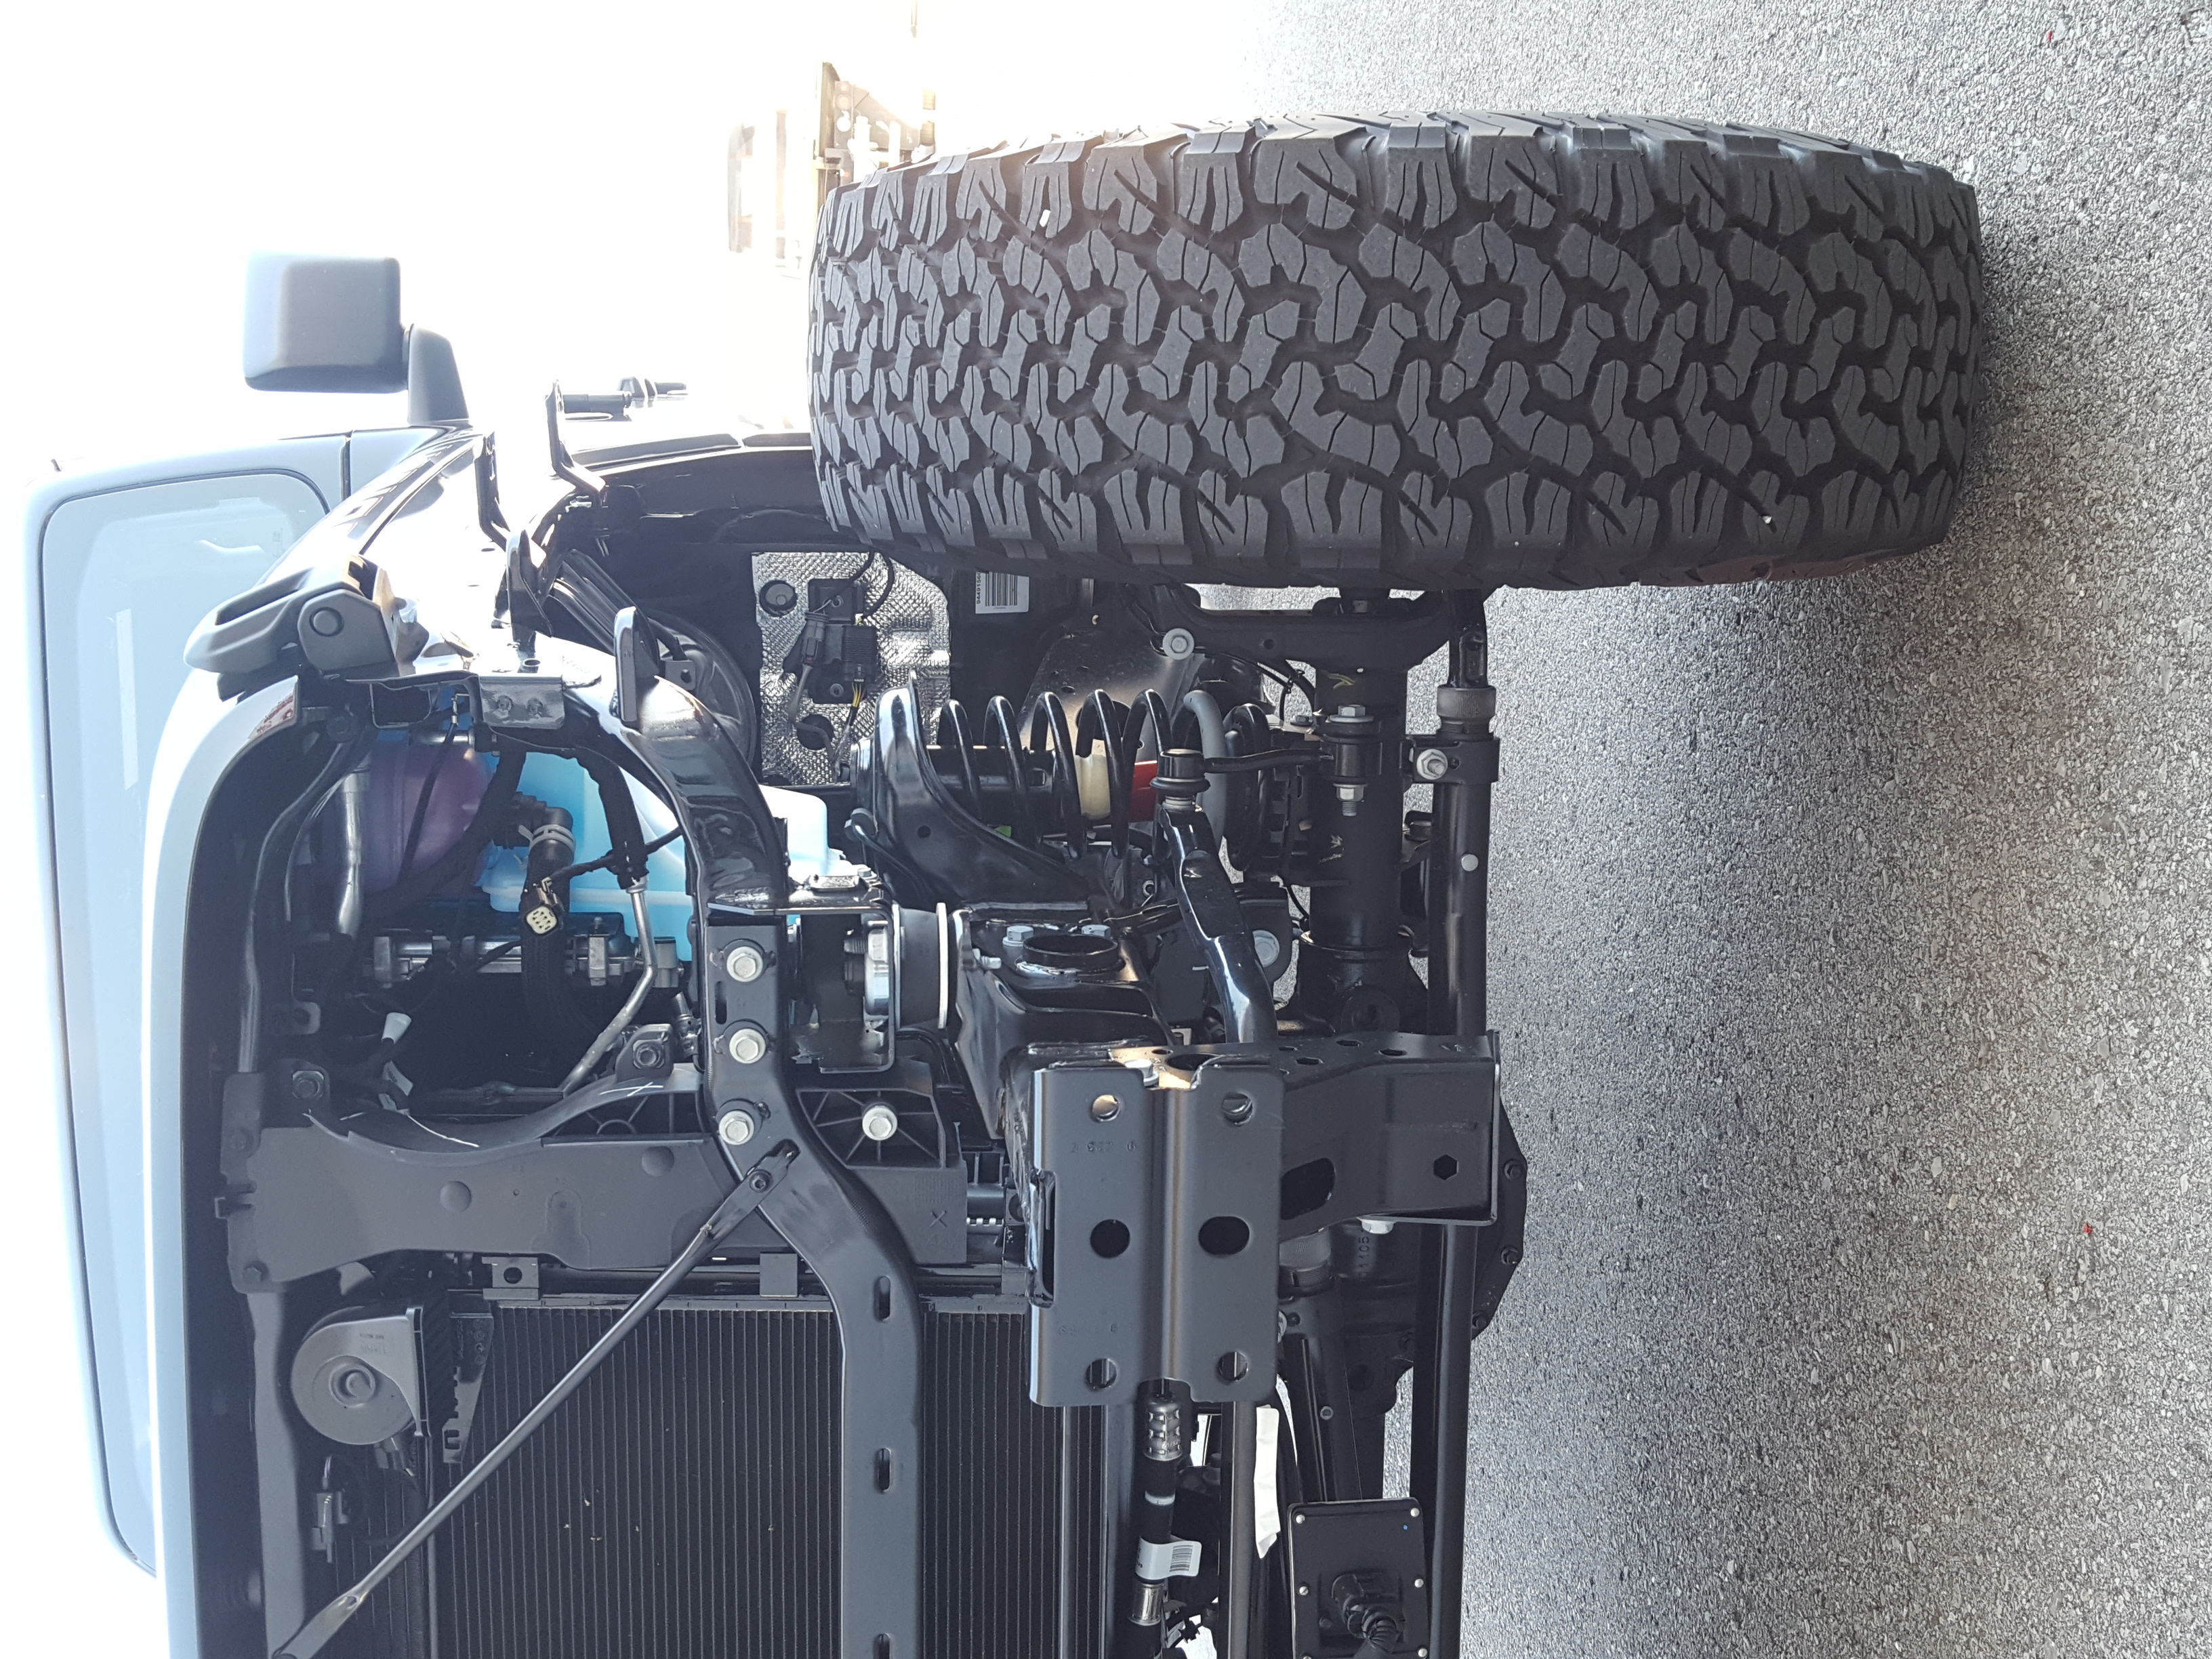
\includegraphics[scale=.1,angle=-90,origin=c]{jeep_01.jpg} 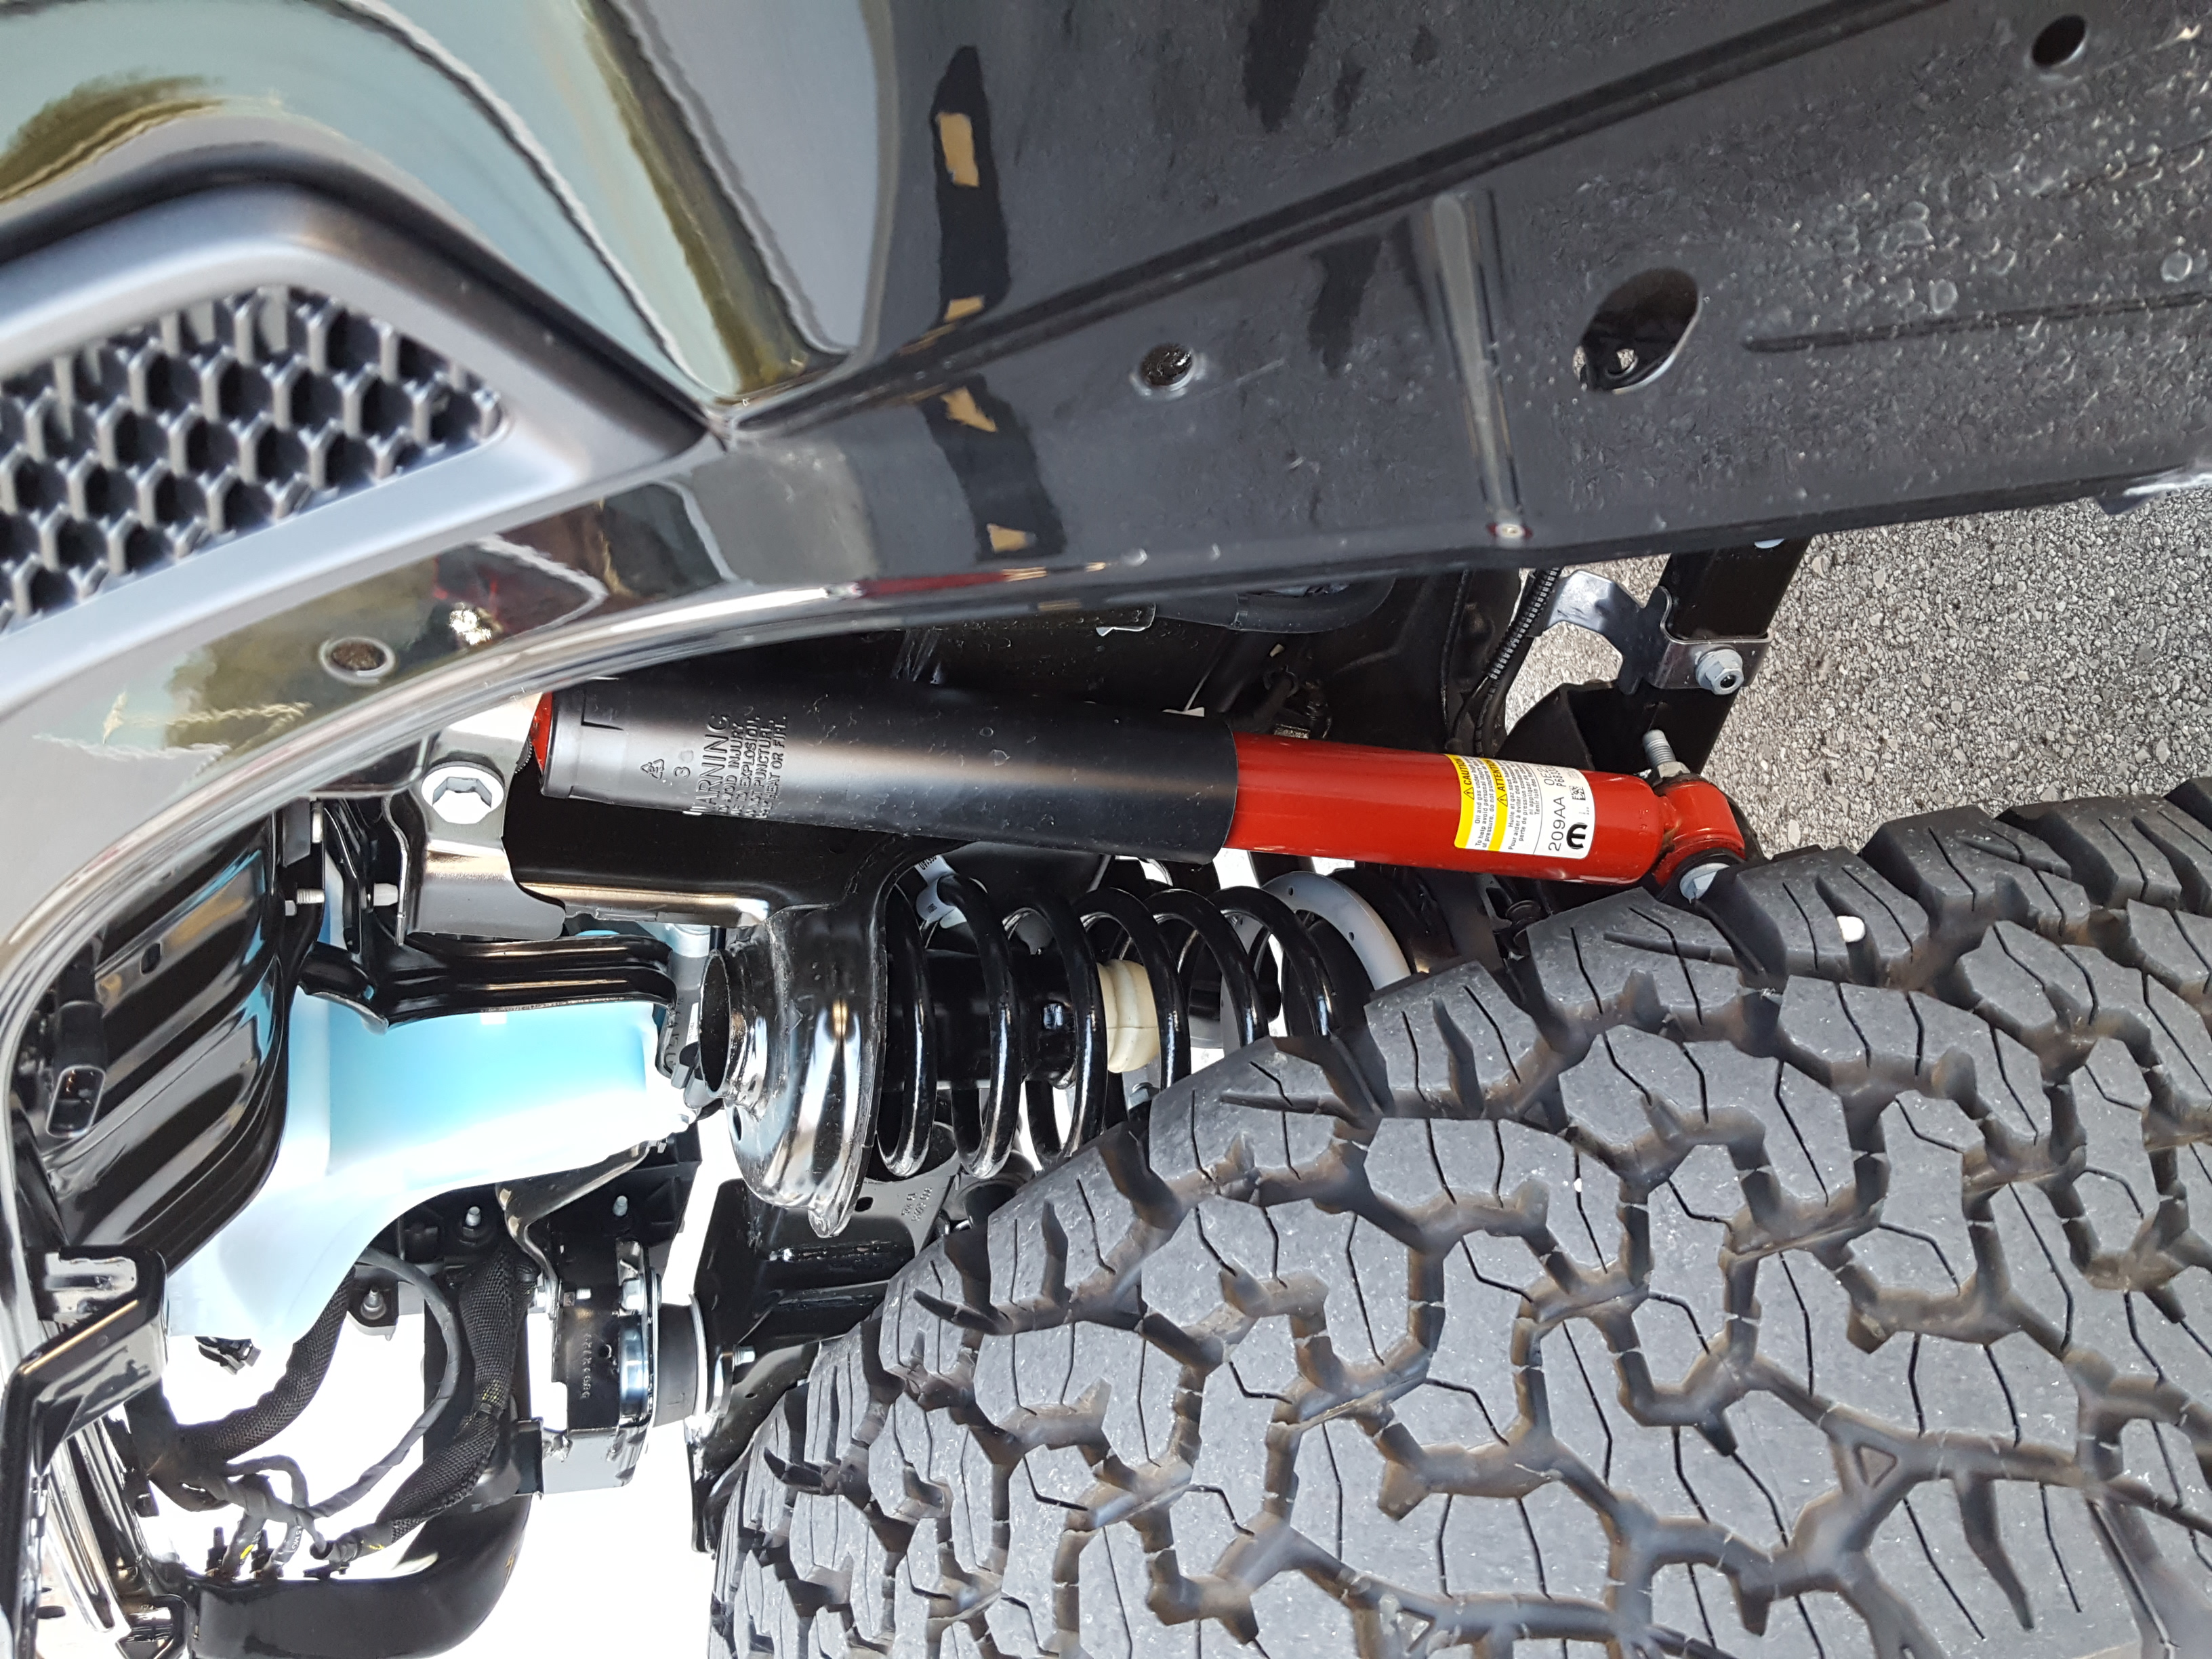
\includegraphics[scale=.1,angle=-90,origin=c]{jeep_02.jpg} \\
%\begin{itemize}
%\item \textbf{ \Large \underline{Problem Statement} -  Derive the \B equations of motion \K using (1) Newton's approach and validate using the (2) Conservation of Energy.}\\
%
%\item \textbf{ \Large \underline{Assumptions} - List the assumptions used in the modeling process.  } 
%
%
%\newpage
%
%\item \textbf{ \Large \underline{Figure(s)} - Draw a \B free body diagram (FBD) \K and/or a sketch of the system. Some problems will require more than one. You need at least one per \B degree of freedom \K.} 
%
%\newpage
%
%\item \textbf{ \Large \underline{Newton's Approach} }\\
%\begin{enumerate}
%\item Draw a Free Body Diagram \vspace{20mm}\\
%\item Determine all \B forces \K acting on the system and their \B directions\K. \vspace{20mm}\\
%\item Write \B Newton's second law \K for the appropriate DOF. \vspace{70mm}\\
%\item Re-write the ODE in the \B standard form \K of a system equation.
%\end{enumerate}
%
%\newpage
%\item \textbf{ \Large \underline{Conservation of Energy Approach} }\\
%\begin{enumerate}
%\item Draw a Free Body Diagram \vspace{20mm}\\
%\item Determine all \B energies \K present in the system and their \B type\K. \vspace{20mm}\\
%\item Write \B Conservation of Energy \K for system. Call this equation 1.\vspace{70mm}\\
%\item Re-write the ODE in the \B standard form \K of a system equation.
%\end{enumerate}
%
%
%\end{itemize}
%
%
%\end{itemize}


	

\end{document}



